% =============================================================================
% Official J.UCS V5 template build of:
% "Accounting for Decision Value: Calibration and Selection over Prediction
%  in a Deployed Equity-Forecasting System."
% Compile with LuaLaTeX (template uses fontspec + Times New Roman):
%     lualatex jucs_decision_value_official.tex   (x2 for refs)
% Requires jucs2e.sty in this folder (copied from the official template).
% =============================================================================
\documentclass[10pt, a4paper, oneside]{article}
\usepackage[hidelinks]{hyperref}
\usepackage{jucs2e}
\usepackage{graphicx}
\usepackage{url}
\usepackage{ulem}
\usepackage{mathtools}
\usepackage{amssymb}
\let\proof\relax\let\endproof\relax
\usepackage{amsthm}
\usepackage{booktabs}
\usepackage{multirow}
\usepackage{enumitem}
\usepackage{scalerel}
\usepackage{setspace}
\usepackage[strict]{changepage}
\usepackage{caption}
\usepackage[letterspace=-50]{microtype}
\usepackage{fontspec}
\usepackage{afterpage}
\usepackage{ragged2e}
\usepackage{tikz}
\usepackage{pgfplots}
\pgfplotsset{compat=1.17}
\usetikzlibrary{arrows.meta,positioning,calc,shapes.geometric,fit,backgrounds}

% Use Times New Roman where it exists (Windows/MiKTeX); otherwise fall back to the
% metric-identical free clone TeX Gyre Termes (e.g. Overleaf/TeX Live on Linux), so the
% file compiles on either. Requires LuaLaTeX or XeLaTeX (fontspec), NOT pdfLaTeX.
\IfFontExistsTF{Times New Roman}{\setmainfont{Times New Roman}}{\setmainfont{TeX Gyre Termes}}

\usepackage{titlesec}
\titleformat*{\section}{\Large\bfseries}
\titleformat*{\subsection}{\normalsize\bfseries}
\titleformat*{\subsubsection}{\normalsize\bfseries\itshape}

\renewcommand{\baselinestretch}{0.9}
\graphicspath{{./figures/}}
\usepackage[textwidth=8cm, margin=0cm, left=4.6cm, right=4.2cm, top=3.9cm, bottom=6.8cm, a4paper, headheight=0.5cm, headsep=0.5cm]{geometry}
\usepackage{fancyhdr}
\usepackage[format=plain, labelfont=it, textfont=it, justification=centering]{caption}
\usepackage{breakcites}
\usepackage{microtype}

\apptocmd{\frame}{}{\justifying}{}
\urlstyle{same}
\pagestyle{fancy}

% --- additions used by the manuscript body -----------------------------------
\theoremstyle{definition}
\newtheorem{definition}{Definition}
\theoremstyle{plain}
\newtheorem{proposition}{Proposition}
\newtheorem{lemma}{Lemma}
\newcommand{\ece}{\mathrm{ECE}}
\newcommand{\Pup}{\hat p}

% --- journal metadata (placeholders; editor assigns final values) ------------
\newcommand\jucs{{Journal of Universal Computer Science}}
\newcommand\jucsvol{vol. XX, no. X (2026)}
\newcommand\jucspages{XXXX-XXXX}
\newcommand\jucssubmitted{XX/XX/2026}
\newcommand\jucsaccepted{XX/XX/2026}
\newcommand\jucsappeared{XX/XX/2026}
\newcommand\jucslicence{ CC BY 4.0}
\newcommand\startingPage{1}
\setcounter{page}{\startingPage}

\newcommand\paperauthor{{Pardeshi, A., Deshmukh, S.: }}
\newcommand\papertitle{Accounting for Decision Value: Calibration and Selection over Prediction in a Deployed Equity-Forecasting System}
\header{\paperauthor Accounting for Decision Value}

% jucs2e hardcodes a sample running head; override its inner-page centre header
% with the real one (vendor jucs2e.sty left unmodified).
\fancyhead[OC]{%
  {\ifnum\thepage=\startingPage
   \begin{singlespace}\fontsize{8pt}{5pt}\selectfont{\itshape{\jucs, \jucsvol, \jucspages \\ submitted: \jucssubmitted, accepted: \jucsaccepted, appeared: \jucsappeared \jucslicence}}\vspace{-5mm}\end{singlespace}
   \else
   \lsstyle{\fontsize{8pt}{5pt}\selectfont{\itshape{Pardeshi, A., Deshmukh, S.: Accounting for Decision Value}}}\vspace{-0.5mm}
   \fi}%
}

\begin{document}

\title{{\fontsize{14pt}{16pt}\selectfont{\vspace*{-3mm}\papertitle\vspace*{-1mm}}}}

\author{{\bfseries\fontsize{10pt}{12pt}\selectfont{Anandkumar Pardeshi}} \\
   {\fontsize{9pt}{11pt}\selectfont{(Department of Computer Science and Engineering, Fr.\ C.\ Rodrigues Institute of Technology,\\
   University of Mumbai, Navi Mumbai, India\\
   \orcid{0000-0002-1825-0097},
   anand.pardeshi@fcrit.ac.in)}}
   \and
   {\bfseries\fontsize{10pt}{12pt}\selectfont{Sujata Deshmukh}}\\
   {\fontsize{9pt}{11pt}\selectfont{(Department of Computer Engineering, Fr.\ C.\ Rodrigues Institute of Technology,\\
   University of Mumbai, Navi Mumbai, India\\
   \orcid{0000-0001-5109-3700},
   sujata.deshmukh@fcrit.ac.in)}}
}

\label{first}
\maketitle

{\fontfamily{ptm}\selectfont
\begin{abstract}
{\fontsize{9pt}{11pt}\selectfont{\vspace*{-2mm}
Most machine-learning work on equity markets is graded on predictive accuracy or
area under the ROC curve, and most of it fails to beat a trivial drift baseline
once costs and look-ahead are handled honestly. We argue that accuracy measures
the wrong thing. What a deployed system delivers is \emph{decision value}: the
quality of the small set of positions it actually takes, weighed against the far
larger set it stays out of. We make this precise by extending the classical
calibration--refinement and reliability--resolution decompositions of forecast
quality to the abstaining, cost-aware decision setting, and we prove a
tail--AUC decoupling result: a one-sided selective rule can earn a positive edge
in its high-conviction tail while global AUC sits at or below one half, so AUC
and accuracy systematically misreport what such a system is worth. We then
\emph{account} for the value of a real deployed system on the Indian National
Stock Exchange across its whole pipeline: multi-source features, a hybrid
gradient-boosted/recurrent ensemble, language-model news scoring, post-hoc
calibration, a conviction gate, and an append-only audit ledger. The numbers are
unforgiving. On 621 resolved forecasts from the live ledger, nominal 90\% price
intervals covered only 70.7\% of outcomes, so deployed confidence was overstated
and self-correcting it was nobody's job. A three-stage recalibration that first
repaired a stacking domain mismatch cut expected calibration error from 0.35 to
0.05 without moving accuracy. Single-name next-period direction was unpredictable
beyond drift (50.1\% out-of-sample, ranking AUC near 0.49). Yet a conviction gate
that abstains on roughly 94\% of names lifted the 30-day hit rate to 60.6\%
against a 58.0\% base (95\% interval 58.8--62.4), positive in four of five test
years. Selection produces the realized edge. Calibration is what makes the gate
trustworthy enough to act on. The predictive model adds almost no ranking alpha.
The practitioner's lesson follows: instrument the uncertainty layer and report
precision at coverage, rather than optimising a number the deployment will not
pay for.}}
\end{abstract}}
{\fontfamily{ptm}\selectfont
\begin{keywords}
{\fontsize{9pt}{11pt}\selectfont{
decision value, calibration, selective prediction,
probabilistic forecasting, financial machine learning, model evaluation, abstention}}
\end{keywords}}
{\fontfamily{ptm}\selectfont
\begin{category}
{\fontsize{9pt}{11pt}\selectfont{
I.2.6, G.3}}
\end{category}}
{\fontfamily{ptm}\selectfont
\begin{doi}
{\fontsize{9pt}{11pt}\selectfont{
10.3897/jucs.\textless SubmissionNumber\textgreater}}
\end{doi}}

\section{Introduction}
\label{sec:intro}
% =============================================================================
A reader who scans the last decade of machine learning applied to stock markets
comes away with a puzzle. Paper after paper reports directional accuracies in the
high fifties or sixties, areas under the ROC curve comfortably above one half, and
backtested Sharpe ratios that would, if real, retire the authors
[Sezer et al.\ 2020, Jiang 2021]. And yet the people who actually run money are not
quietly compounding these edges away in private. The gap between the published
record and the deployed reality is wide enough that something in how the field
keeps score must be wrong.

We think the something is the scorecard itself. Accuracy and AUC answer a question
about \emph{ordering}: given two names, does the model tend to rank the one that
rose above the one that fell? That question has a clean answer and a long
literature, and it is almost the wrong question for a system that has to decide,
name by name, day by day, whether to put on a position or stay flat. A deployed
forecaster does not grade every name. It commits to a few and abstains on the rest,
and its worth is the quality of the commitments, weighed against the cost of the
ones it skipped. Call this \emph{decision value}. Decision value is not accuracy,
nor is it a monotone function of AUC. The uncomfortable part is that a system can
have real decision value while its accuracy and AUC report none.

This paper is an exercise in accounting for decision value, carried out on a real
system rather than a toy. The system is a production equity-forecasting platform
for liquid large capitalisations on the National Stock Exchange of India (NSE),
built around the components that have become standard practice: a multi-source
feature stack over price, momentum, trend, mean reversion and volatility; a hybrid
ensemble that blends gradient-boosted trees with a recurrent sequence model; a
language-model layer that scores news; a post-hoc calibration stage; a conviction
gate that decides when to act; and an append-only ledger that records every issued
forecast so that the system can be graded against the future it actually faced.
The platform is live, it has two user-facing surfaces, and since April 2026 it has
been writing down what it predicts so that nobody, including its authors, can quietly
rewrite the past.

What we found in the live record is worth stating up front, because it sets
the agenda for the rest of the paper. First, the deployed uncertainty was wrong in
a measurable, one-directional way: nominal 90\% price intervals contained the
realised price only 70.7\% of the time over 621 resolved forecasts, and nothing in
the pipeline was responsible for noticing. Second, the model's calibration could be
repaired. Expected calibration error fell from 0.35 to 0.05, and the repair added no
accuracy; it only pulled the probabilities back onto what the data supported. Third,
once the probabilities were trustworthy, the directional skill that the
miscalibration had been hiding turned out not to exist: at short horizons,
single-name direction across this universe is unpredictable beyond the upward drift
of equities, with out-of-sample accuracy at 50.1\% and ranking AUC near 0.49.
Fourth, and the reason the system is nonetheless useful, a conviction gate that
keeps quiet on roughly 94\% of names earns a small but repeatable edge on the few it
flags: a 60.6\% thirty-day hit rate against a 58.0\% base, holding up in four of
five test years.

Read as accuracy figures these results are a catalogue of failures. Read as a
decision-value account they tell a coherent and, we will argue, generalisable
story. The predictive model contributes almost none of the realised value. What
value there is comes from \emph{selection}, the discipline of acting only in the
high-conviction tail, and calibration is what lets the conviction threshold mean
what it says. Drift is beta, not skill. The ranking signal that accuracy and AUC
are built to reward is, here, absent. Graded on the usual scorecard, the system
looks worthless. Graded on the value it can be paid for, it shows a thin but real
edge, and you can point to the component responsible.

\subsection{Contributions}
\label{sec:contrib}
The paper makes three contributions, one conceptual, one theoretical, and one
empirical.

\begin{enumerate}[leftmargin=1.4em,itemsep=2pt,topsep=2pt]
\item \emph{A decision-value accounting framework} (Section~\ref{sec:framework}).
We define the decision value of a selective, cost-aware forecaster and decompose it
into a drift (base-rate) term, a selection (refinement) term realised at a
conviction threshold, and a calibration term that enables rather than adds. The
decomposition is the selective-prediction counterpart of the calibration--refinement
partition of [DeGroot and Fienberg 1983] and the reliability--resolution partition
of [Murphy 1973], and it makes ``where does the value come from'' a question with a
measurable answer.
\item \emph{A tail--AUC decoupling result} (Section~\ref{sec:tail}). We prove that
the selection term is a property of the extreme tail of the score distribution and
is largely independent of global ordering: there exist score--label distributions
with AUC no greater than one half on which a one-sided conviction rule still earns a
strictly positive tail edge. The practical consequence is that AUC and accuracy can
report zero skill on a system that has decision value, which is the regime we
then measure, and it is why precision at a fixed firing rate is the right instrument.
\item \emph{A whole-system attribution on a deployed platform}
(Sections~\ref{sec:system}--\ref{sec:results}). We instrument a live system and
report measured numbers only: live-ledger interval coverage, a calibration repair
that traces to a concrete stacking bug, a verified accuracy ceiling established five
ways, and a walk-forward selective signal over eight years. We then carry out the
attribution, separating the contribution of drift, calibration, selection and
ranking, and showing that ranking contributes essentially nothing while selection
carries the system.
\end{enumerate}

We are careful about scope throughout, in keeping with a standing
rule on this project that no reported number is synthetic. Where the live ledger
cannot support a claim (most importantly, an isolated return attributable to the
news layer, for which per-event labels are not stored), we say so and argue from
structure and from the measured end-to-end behaviour instead of manufacturing a
clean figure. Section~\ref{sec:discussion} returns to these limits.

% =============================================================================
\section{Related work}
\label{sec:related}
% =============================================================================
\noindent\textbf{Machine learning for markets, and how it is graded.}
Deep and ensemble models for equity prediction are now routine. Long short-term
memory networks [Fischer and Krauss 2018], gradient-boosted trees and random forests
for statistical arbitrage [Krauss et al.\ 2017], and large cross-sectional studies of
machine-learning asset pricing [Gu et al.\ 2020] are representative, and two
systematic reviews map the territory [Sezer et al.\ 2020, Jiang 2021]. The dominant
evaluation currency in this literature is directional accuracy or AUC, sometimes a
backtested Sharpe ratio. A parallel and more sceptical methodological line has shown
how fragile those currencies are: backtest overfitting inflates apparent performance
[Bailey et al.\ 2017], the cross-section of ``discovered'' predictors is riddled with
multiple-testing artefacts [Harvey et al.\ 2016], and a careful treatment of leakage,
costs and capacity removes most reported edges [Lopez de Prado 2018]. Our paper sits
inside this sceptical line but turns it constructive: rather than only warn that the
usual scorecard misleads, we replace it with a decision-value account and show what
the account reveals on a system we operate.

\noindent\textbf{Calibration of probabilistic forecasts.}
Modern classifiers are frequently overconfident [Guo et al.\ 2017]. The standard
post-hoc remedies are Platt scaling [Platt 1999] and isotonic regression
[Zadrozny and Elkan 2002], with reliability assessed by the expected calibration
error [Naeini et al.\ 2015] and the Brier score [Brier 1950, Niculescu-Mizil and
Caruana 2005]. The foundational decompositions of forecast quality are older and,
for our purposes, central: [Murphy 1973] partitions the Brier score into reliability,
resolution and uncertainty, and [DeGroot and Fienberg 1983] partition forecaster
quality into calibration and refinement. [Gneiting et al.\ 2007] crystallise the
operating principle these decompositions imply (maximise sharpness subject to
calibration), which is the thesis of this paper carried into the decision setting.
We use these results as the scaffolding of our framework, not merely as background.
A known trap when calibration meets stacked generalisation
[Wolpert 1992] is that a calibrator fitted on one stage's scores and applied to
another silently fails. We diagnose this failure in Section~\ref{sec:cal}.

\noindent\textbf{Selective prediction and abstention.}
Allowing a model to decline to answer is an old idea [Chow 1970] with a modern
theory of risk--coverage trade-offs [El-Yaniv and Wiener 2010, Geifman and El-Yaniv
2017] and a distribution-free cousin in conformal prediction [Vovk et al.\ 2005,
Angelopoulos and Bates 2021], including variants built for the non-stationary
coverage failures we observe [Gibbs and Cand\`es 2021]. This community measures
risk at a given coverage; the financial-ML community, by contrast, rarely reports
whether its probabilities are trustworthy or whether the model knows when to stay
out. Our decision-value framework argues that the selective
view is the correct one for deployed financial systems, and makes that argument
quantitative on a real deployment. The closest framing in spirit treats trustworthy financial AI as an
abstention problem; we differ by making the object of study the \emph{attribution}
of value across pipeline stages rather than a prescriptive contract, and by
supplying the tail--AUC result that explains why the attribution comes out as it
does.

\noindent\textbf{Text and returns.}
That media content carries return-relevant information is well established
[Tetlock 2007, Antweiler and Frank 2004], that finance-specific dictionaries matter
because general ones mislabel domain terms is the lesson of [Loughran and McDonald
2011], and supervised or pre-trained language models now dominate sentiment
extraction [Devlin et al.\ 2019, Ke et al.\ 2019]. Whether instruction-tuned models
can read financial news and anticipate moves is under active study [Lopez-Lira and
Tang 2023]. Our system uses a language model as one feature source; we are careful,
in Section~\ref{sec:results}, not to claim an isolated alpha for it that our ledger
cannot support.

\noindent\textbf{Forecast value and decision-theoretic evaluation.}
A separate tradition asks not whether a forecast is accurate but whether it is
\emph{useful}: what a decision-maker gains by acting on it. Murphy [Murphy 1993]
separated the consistency, quality, and value of a forecast and argued that the three
need not move together, an older statement of our complaint that a high AUC need not
become a usable signal. Granger and Pesaran [Granger and Pesaran 2000] sharpened the
point for economics, showing that a statistical loss function and the economic payoff
of a decision can rank forecasters in different orders. Proper scoring rules formalise
when honest probabilities are rewarded [Gneiting and Raftery 2007], and in finance the
realised worth of a strategy is usually read off a risk-adjusted return such as the
Sharpe ratio [Sharpe 1994]. Decision value belongs to this lineage. It is a value
measure, conditioned on a cost-aware action rule, rather than a quality measure
averaged over every forecast. What we add is a decomposition of that value into named,
separately measurable parts, and a theorem about why the quality measures cannot see
it.

Our paper sits at the meeting point of three literatures that rarely talk to each
other: the score decompositions of forecast verification, the risk--coverage view
of selective prediction, and a financial-ML literature that has learned to distrust
its own evaluations. We weld them into an attribution method and run it on a live
system.

% =============================================================================
\section{A decision-value accounting framework}
\label{sec:framework}
% =============================================================================
This section sets up the bookkeeping. We define the value a selective forecaster
delivers, decompose it into interpretable terms, and prove the result that makes the
decomposition necessary rather than cosmetic: that the actionable term lives in the
tail and is invisible to AUC.

\subsection{Forecasts, decisions, and decision value}
\label{sec:defs}
Fix a horizon of $H$ trading days. For each name and date the system emits a
calibrated directional probability $\Pup\in[0,1]$ that the $H$-day forward return is
positive, together with a point forecast and a price interval. Let $y\in\{0,1\}$ be
the realised direction. A \emph{one-sided selective rule} $d_\tau$ acts, taking a long
position for the horizon, when $\Pup\ge\tau$ and abstains otherwise. We focus on the
one-sided long/abstain rule because, as Section~\ref{sec:ceiling} shows empirically,
confident short calls on single names are destroyed by drift; nothing in the
framework requires one-sidedness.

Two quantities summarise the rule's behaviour. Its \emph{firing rate}
$\phi(\tau)=\Pr[\Pup\ge\tau]$ is the fraction of opportunities on which it acts, and
its \emph{fired precision} $\pi(\tau)=\Pr[y=1\mid \Pup\ge\tau]$ is the realised up-rate
among the positions it takes. Let $b=\Pr[y=1]$ be the unconditional up-rate, the
base that a name-blind ``always act'' policy would achieve.

\begin{definition}[Selection value and decision value]
\label{def:dv}
The \emph{selection value} of the rule $d_\tau$ is the edge of its fired positions
over the base,
\begin{equation}
\label{eq:sigma}
\sigma(\tau)\;=\;\pi(\tau)-b .
\end{equation}
Its \emph{decision value} at firing rate $\phi$ is the selection value scaled by how
often the rule is willing to act and net of the per-trade cost $\kappa$ of acting,
\begin{equation}
\label{eq:dv}
V(\tau)\;=\;\phi(\tau)\,\big[\,g\,\sigma(\tau)-\kappa\,\big],
\end{equation}
where $g$ converts a unit of directional edge into a unit of payoff for the position
sizing in use.
\end{definition}

Equation~\eqref{eq:dv} is intentionally minimal: the realised worth of a selective
forecaster is set by how often it acts, how much its acted-upon calls beat the base,
and what acting costs. Nothing else enters. Neither accuracy nor AUC appears in it.
A model can be excellent on both and still have $V\le 0$ when its edge does not
survive cost; a model at chance on both can have $V>0$ if it finds a thin, reliable
tail. The cost $\kappa$ and the sizing factor $g$ are venue-specific, so the
empirical attribution of Section~\ref{sec:results} concentrates on the cost-free core
of $V$ (the selection value $\sigma$) and returns to the net-of-cost picture once
$\sigma$ has been measured (Section~\ref{sec:swing}). The rest of the framework is
about where $\sigma$ comes from and why the usual metrics cannot see it.

\subsection{Decomposing fired precision}
\label{sec:decomp}
The fired precision admits a decomposition that mirrors the classical partitions of
forecast quality but is conditioned on the act region rather than averaged over all
forecasts. Write the act region as $R_\tau=\{\Pup\ge\tau\}$ and let
$\bar p(\tau)=\mathbb E[\Pup\mid R_\tau]$ be the mean predicted probability there.
Adding and subtracting $\bar p(\tau)$ in \eqref{eq:sigma},
\begin{equation}
\label{eq:partition}
\underbrace{\pi(\tau)-b}_{\text{selection value }\sigma(\tau)}
\;=\;
\underbrace{\big(\pi(\tau)-\bar p(\tau)\big)}_{\text{calibration gap on }R_\tau}
\;+\;
\underbrace{\big(\bar p(\tau)-b\big)}_{\text{conviction lift}} .
\end{equation}
The second term, the conviction lift, is how far above the base the model is willing
to claim on its acted-upon names; it is pure refinement, the analogue of resolution
in [Murphy 1973]. The first term, the calibration gap, is how wrong that claim turns
out to be on those same names; under perfect calibration it is zero and the realised
edge equals the claimed lift. Miscalibration enters \emph{only} through this term: a
model that systematically over-claims has a negative calibration gap that eats into,
or reverses, the lift it advertises. Calibration here enables the edge without adding
to its size. It does not generate conviction lift, which is a property of how the
model ranks opportunities. But when it is broken, the lift on paper is not the edge
you collect, and the threshold $\tau$ stops meaning what you set it to.

The decomposition also explains why repairing calibration can leave accuracy
untouched while transforming a system's usability. A monotone recalibration map (Platt
or isotonic) is order-preserving, so it moves neither accuracy nor AUC nor the
conviction lift $\bar p(\tau)-b$ evaluated at the matched quantile; a non-monotone
calibrator could reorder names and would carry no such guarantee. What the monotone
map moves is the calibration gap, pulling $\bar p(\tau)$ back onto $\pi(\tau)$ so that
the advertised probability equals the delivered one. Section~\ref{sec:resultcal} shows
this happening to a real model.

\subsection{Relation to the Brier-score decomposition}
\label{sec:brier}
The two terms in \eqref{eq:partition} are the act-region shadows of a classical
result. Murphy [Murphy 1973] split the Brier score of a probabilistic forecaster into
three pieces,
\begin{equation}
\label{eq:murphy}
\mathrm{BS}=\underbrace{\mathbb{E}\big[(\bar p_{\text{bin}}-\bar y_{\text{bin}})^2\big]}_{\text{reliability}}
-\underbrace{\mathbb{E}\big[(\bar y_{\text{bin}}-b)^2\big]}_{\text{resolution}}
+\underbrace{b(1-b)}_{\text{uncertainty}},
\end{equation}
where the expectations run over the forecaster's probability bins, $\bar y_{\text{bin}}$
is the realised rate in a bin, and $b$ is the base rate. Reliability is small when the
forecaster is calibrated; resolution is large when its bins pull outcomes apart; the
uncertainty term depends only on the base rate, never on the model. A conviction gate
keeps a single bin, the act region $R_\tau$, and reads two of these three quantities
in \eqref{eq:murphy} through it. The conviction lift $\bar p(\tau)-b$ of \eqref{eq:partition} is the local
face of resolution: a forecaster with no resolution cannot push its acted-on
probabilities above the base, so the gate has nothing to fire on. The calibration gap
$\pi(\tau)-\bar p(\tau)$ is the local face of reliability, and the expected calibration
error of \eqref{eq:ece}, defined in Section~\ref{sec:cal}, is its size summed over
bins. This is the formal reason the
attribution falls out the way it does. Selection value is resolution restricted to the
tail; calibration is reliability; and the base rate, the uncertainty term, is the drift
that neither the model nor the gate may claim. We record the correspondence as a lemma.

\begin{lemma}[Local resolution and reliability]
\label{lem:res}
Fix $\tau$ and treat the act region $R_\tau$ as one bin, with mean forecast
$\bar p(\tau)$ and realised rate $\pi(\tau)$. The selection value splits as
$\sigma(\tau)=\big(\pi(\tau)-\bar p(\tau)\big)+\big(\bar p(\tau)-b\big)$, a local
reliability gap plus a local resolution lift. If the underlying forecaster has zero
resolution, so that its realised positive rate equals the base $b$ on every set fixed
by the forecast value, then $\pi(\tau)=b$ for every threshold $\tau$, and therefore
$\sigma(\tau)=0$: no gate can extract an edge.
\end{lemma}
\begin{proof}
The split is \eqref{eq:partition} with $\bar p(\tau)=\mathbb{E}[\Pup\mid R_\tau]$. Zero
resolution means the realised rate is $b$ on every event determined by the forecast
value; $R_\tau=\{\Pup\ge\tau\}$ is such an event, so $\pi(\tau)=\Pr[y=1\mid R_\tau]=b$,
whence $\sigma(\tau)=\pi(\tau)-b=0$.
\end{proof}

Lemma~\ref{lem:res} says a gate cannot manufacture an edge from a forecaster that does
not separate outcomes. All it can do is harvest whatever resolution exists, which sits
in the tail, and only if calibration is good enough that the tail is where the
forecaster claims it is. That proviso is the entire job of the calibration repair in
Section~\ref{sec:resultcal}.

\subsection{Selection lives in the tail: a decoupling from AUC}
\label{sec:tail}
A decision-value account would just relabel the usual numbers if its central term
tracked them. It does not. The selection value can be positive when AUC reports no
signal at all. AUC is a global statistic, the probability that a random positive
outscores a random negative, and it averages concordance over the whole score
distribution. Selection value, by \eqref{eq:sigma}, depends only on the conditional
up-rate inside a thin top slice. The two can come apart, and on real market data they
do.

\begin{proposition}[Tail--AUC decoupling]
\label{prop:tail}
For every $\varepsilon\in(0,\tfrac12)$ and every $\sigma_0\in(0,\,1-b)$ there is a
joint distribution of a score $S$ and label $Y\in\{0,1\}$ with base rate
$\Pr[Y=1]=b$ such that, for the threshold $\tau$ with firing rate $\phi(\tau)=\varepsilon$,
the selection value satisfies $\sigma(\tau)\ge\sigma_0$, while the global
$\mathrm{AUC}(S,Y)\le \tfrac12$.
\end{proposition}

\begin{proof}
We construct such a distribution explicitly. Put all score mass on three cells,
ordered $B_1 < B_2 < T$ by score, with ties allowed only within a cell. The top cell
$T$ has mass $\varepsilon$ and conditional positive rate $b+\sigma_0$ (a valid
probability since $\sigma_0<1-b$); the two bulk cells $B_1,B_2$ each have mass
$m=(1-\varepsilon)/2$ and positive rates $p_1=b+a$ and $p_2=b-c$. The threshold
$\tau=\inf T$ fires on exactly $T$, so $\phi(\tau)=\varepsilon$ and
$\pi(\tau)=b+\sigma_0$, hence $\sigma(\tau)=\sigma_0$. Holding the overall base at $b$
requires $\varepsilon(b+\sigma_0)+m(p_1+p_2)=b$, i.e.
\begin{equation}
\label{eq:basecon}
a-c=-\frac{2\varepsilon\sigma_0}{1-\varepsilon}.
\end{equation}
The bulk is \emph{anti-sorted} when $p_1>p_2$ (equivalently $a+c>0$): the
higher-scored cell $B_2$ carries the lower positive rate.

Write the AUC as the probability that a random positive outscores a random negative,
ties counted as one half, and let $P=b$, $N=1-b$ be the total positive and negative
mass. Let $(t_1,t_0)=\varepsilon(b+\sigma_0,\,1-b-\sigma_0)$ be the positive and
negative mass of $T$, and likewise $(u_1,u_0)=m(p_2,1-p_2)$ for $B_2$ and
$(v_1,v_0)=m(p_1,1-p_1)$ for $B_1$. Summing concordance over ordered cell pairs, where
a positive--negative pair is concordant when the positive's cell has the higher score,
scores one half within a shared cell, and zero otherwise, gives
\begin{equation}
\label{eq:aucsum}
\mathrm{AUC}\cdot PN
=\underbrace{t_1(u_0+v_0)+u_1 v_0}_{\text{concordant}}
+\tfrac12\underbrace{\big(t_1 t_0+u_1 u_0+v_1 v_0\big)}_{\text{within-cell ties}} .
\end{equation}
The discordant pairs (a positive scored below its negative, chiefly the large mass
$v_1 u_0$ in which a $B_1$ positive sits below a $B_2$ negative) contribute zero, and
this is where the anti-sorted bulk pays. The two tail terms $t_1(u_0+v_0)$ are
$O(\varepsilon)$. Raising the bulk contrast $c$, with $a$ following by
\eqref{eq:basecon}, drives $p_2\!\downarrow$ and $p_1\!\uparrow$ and lowers the
right-hand side of \eqref{eq:aucsum}; the contrast is feasible up to $p_2=b-c\ge 0$.
For any fixed $\varepsilon,\sigma_0$ a large enough bulk deficit therefore dominates the
$O(\varepsilon)$ tail surplus, giving $\mathrm{AUC}\le\tfrac12$ while $\sigma(\tau)=\sigma_0$.

A concrete instance settles existence. Take $b=\tfrac12$, $\sigma_0=0.2$,
$\varepsilon=0.1$, and $c=0.4$, so by \eqref{eq:basecon} $a=0.356$, giving $p_1=0.856$,
$p_2=0.1$, and a top rate $b+\sigma_0=0.7$. Then $t_1=0.07,\,t_0=0.03$;
$u_1=0.045,\,u_0=0.405$; $v_1=0.385,\,v_0=0.065$, and \eqref{eq:aucsum} evaluates to
$0.07(0.405{+}0.065)+0.045(0.065)+\tfrac12(0.0021{+}0.0182{+}0.0250)=0.0585$, so
$\mathrm{AUC}=0.0585/0.25=0.234\le\tfrac12$, while the gate earns $\sigma(\tau)=0.2$ at
firing rate $\phi=0.1$.
\end{proof}

\begin{figure}[t]
\centering
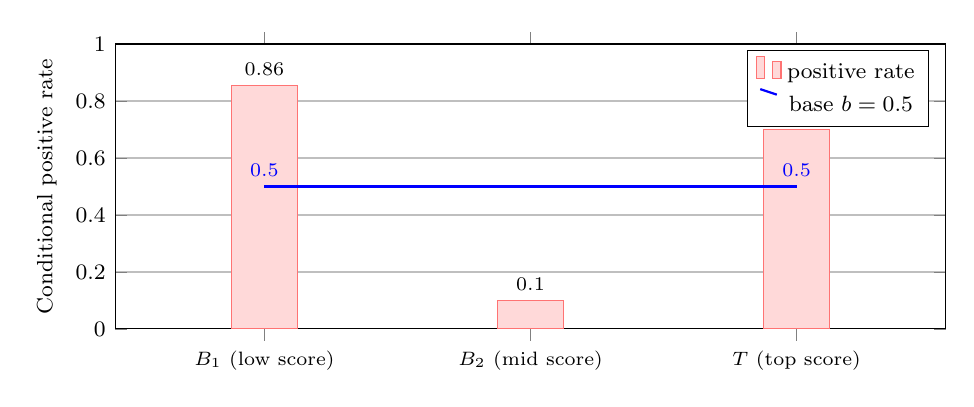
\begin{tikzpicture}
\begin{axis}[
  width=\linewidth, height=5.2cm, font=\footnotesize,
  ybar, bar width=24pt,
  symbolic x coords={$B_1$ (low score),$B_2$ (mid score),$T$ (top score)},
  xtick=data, x tick label style={font=\scriptsize},
  ymin=0, ymax=1, ylabel={Conditional positive rate},
  enlarge x limits=0.28, ymajorgrids,
  nodes near coords, every node near coord/.append style={font=\scriptsize},
]
\addplot[fill=red!15,draw=red!55] coordinates {($B_1$ (low score),0.856)($B_2$ (mid score),0.1)($T$ (top score),0.7)};
\addplot[sharp plot,thick,blue,mark=none,update limits=false] coordinates {($B_1$ (low score),0.5)($T$ (top score),0.5)};
\legend{positive rate, base $b=0.5$}
\end{axis}
\end{tikzpicture}
\caption{The tail--AUC construction of Proposition~\ref{prop:tail}, drawn for the
worked instance ($b=\tfrac12$, $\sigma_0=0.2$, $\varepsilon=0.1$, $c=0.4$). The bulk is
anti-sorted: the low-score cell $B_1$ carries a high positive rate while the mid-score
cell $B_2$ carries a low one, which drags global AUC down to $0.234$. The thin top cell
$T$ still sits above the base, so a gate firing only on $T$ banks $\sigma=0.2$. The
figure illustrates the construction and makes no empirical claim.}
\label{fig:construction}
\end{figure}

The construction is not a curiosity (Figure~\ref{fig:construction}). A system whose scores are slightly
anti-informative in the bulk (common when a model has learned a weak mean-reverting
pattern that is wrong on average but concentrates a few genuine signals at the
extreme) will report $\mathrm{AUC}\le\tfrac12$ and look worthless, while a conviction
gate reading only its top few per cent collects a real edge. The standard scorecard
does not merely understate such a system; it can assign it a failing grade. What does
see the edge is precision at a fixed firing rate, $\pi(\tau)$ at $\phi(\tau)$, the
quantity our results report and the attribution in Section~\ref{sec:attrib} is built
on. None of this makes AUC meaningless. For ranking-driven applications it is the
right tool. It is the wrong instrument for a selective decision system, and the
proposition is why.

\subsection{The attribution procedure}
\label{sec:procedure}
The framework yields a procedure that we apply to the deployed system in
Section~\ref{sec:results}. Given a held-out, walk-forward stream of
$(\Pup,y)$ pairs and the live ledger of resolved intervals, the decision-value
attribution is:
\begin{enumerate}[leftmargin=1.4em,itemsep=2pt,topsep=2pt]
\item \emph{Audit deployed uncertainty.} On the live ledger, compare nominal interval
coverage to empirical coverage. A gap establishes that confidence is not
self-correcting and fixes the stakes (Section~\ref{sec:resultcov}).
\item \emph{Measure the calibration term.} Compute $\ece$ before and after
recalibration; verify that accuracy and AUC are unchanged, isolating the calibration
gap of \eqref{eq:partition} as the only thing that moved (Section~\ref{sec:resultcal}).
\item \emph{Bound the ranking term.} Estimate AUC and accuracy directly to establish
whether any global ordering skill exists (Section~\ref{sec:ceiling}).
\item \emph{Measure the selection term.} Tune the conviction threshold $\tau^\star$ on
training folds, then report $\pi(\tau^\star)$, $\phi(\tau^\star)$ and
$\sigma(\tau^\star)$ out-of-sample with a confidence interval and a test against the
base (Section~\ref{sec:swing}).
\item \emph{Settle the attribution.} Express the realised fired precision as
$b+\sigma(\tau^\star)$ and attribute each component, contrasting it with the
ranking-based reading the standard scorecard would give (Section~\ref{sec:attrib}).
\end{enumerate}
The output is a single accounting that says, in measured numbers, which part of a
machine-learning pipeline is doing the paying.

% =============================================================================
\section{The deployed system and the evaluation protocol}
\label{sec:system}
% =============================================================================
The framework is general; the numbers in Section~\ref{sec:results} come from one
concrete system, which we describe here in enough detail to make the measurements
reproducible in spirit. The platform is a live equity decision-support product for
the Indian NSE. It runs as two surfaces over a shared model and service layer: a
research-facing analytics application and a user-facing web application with a
separate forecasting backend. Both read the same trained artefacts, so the numbers in
this paper describe the models that real users see.

\subsection{Signals, features, and the hybrid ensemble}
\label{sec:ensemble}
For each name the system builds a daily feature stack from end-of-day price data:
returns over several look-backs, momentum and trend descriptors, mean-reversion
indicators, and realised-volatility measures. On top of this it maintains a news
layer (Section~\ref{sec:news}) that scores recent headlines for each entity. These
features feed a \emph{hybrid ensemble} that blends two model families with
complementary inductive biases: a gradient-boosted tree ensemble that captures
threshold and interaction structure in the cross-section, and a recurrent sequence
model over the price history that captures temporal dependence. The two are combined
by a learned blend; the ensemble emits, per name and horizon, a point forecast, a
price interval at a nominal confidence level, and a directional probability $\Pup$.

We treat the ensemble as a black box for the purposes of this paper. That is not
laziness; it is the point. The decision-value account does not care how the
probability was produced, only whether it is calibrated and whether the system knows
when to trust it. The components that determine those two properties, the calibration
stage and the conviction gate, sit downstream of the ensemble, and that is where the
analysis concentrates.

\subsection{News as a feature: a language model as measurement instrument}
\label{sec:news}
The news layer scores each recent headline for an entity and folds the result into
the feature stack. Scoring is done by a compact instruction-tuned language model
(in the current deployment, Claude Haiku 4.5 from Anthropic), prompted as a
quantitative analyst and constrained to emit structured numeric judgements with
fixed numerical anchors so that two runs on the same item agree closely. Each scored
item is memoised in a content-addressed cache keyed by a hash of the entity and the
normalised headline, so a given headline is scored once and reused; when the model is
unavailable a transparent lexicon fallback supplies a conservative score that is
flagged for downstream consumers. We describe the news layer because it is part of the
deployed system and because the journal asks that any use of AI tools be disclosed
(see also the declaration at the end of the paper). We do \emph{not}, however, claim a
standalone return for it: the live ledger does not store per-event return labels, so an
isolated news alpha is not identifiable from our deployment, and we decline to
reconstruct one. Its role in this paper is as one input to the ensemble whose
end-to-end behaviour we measure.

\subsection{Calibration stage}
\label{sec:cal}
A directional probability is only useful if it is calibrated: among names assigned
$\Pup\approx0.7$, about 70\% should rise. We measure calibration by the expected
calibration error over $B$ equal-width bins,
\begin{equation}
\label{eq:ece}
\ece=\sum_{b=1}^{B}\frac{|G_b|}{N}\,\big|\,\overline{y}_b-\overline{p}_b\,\big|,
\end{equation}
where $\overline{p}_b$ and $\overline{y}_b$ are the mean predicted probability and mean
realised outcome in bin $b$, complemented by the Brier score
$\tfrac1N\sum_i(\Pup_i-y_i)^2$ [Brier 1950]. The calibration stage applies a learned
monotone map to the ensemble's raw directional score. Section~\ref{sec:resultcal}
documents what happened when we first measured \eqref{eq:ece} on the deployed model.
It was badly broken, and the bug was the system's own.

\subsection{The conviction gate}
\label{sec:gate}
Calibration makes $\Pup$ honest; it does not make it skilful. If short-horizon
single-name direction is near-random, a calibrated probability sits near the base rate
almost everywhere, and acting on every name is pointless. The conviction gate is the
one-sided selective rule $d_\tau$ of Section~\ref{sec:defs}: for horizon $H$ it emits
an UP call when $\Pup\ge\tau^\star$ and NEUTRAL otherwise. The threshold is tuned on
training folds as the smallest $\tau$ whose fired bucket reaches a target precision
$p_0$ while still firing at least a minimum fraction $\phi_0$ of the time,
\begin{equation}
\label{eq:tau}
\tau^\star=\min\big\{\tau:\ \pi(\tau)\ge p_0\ \text{and}\ \phi(\tau)\ge\phi_0\big\},
\end{equation}
with $p_0=0.60$ and $\phi_0=0.05$ in deployment. The gate is intentionally one-sided
for the empirical reason given in Section~\ref{sec:ceiling}. Choosing $\tau^\star$ on
training data and reporting $\pi,\phi$ out-of-sample is what keeps the selection-value
estimate honest; this is the threshold-tuning analogue of not peeking at the test set.

\subsection{The append-only audit ledger}
\label{sec:ledger}
Since April 2026 the deployed system has written every issued forecast to an
append-only ledger: entity, issue timestamp, target date, point forecast, interval,
nominal confidence, directional probability and horizon. Each row is later stamped
with the realised price and outcome on its original target date and is never
retro-edited; scoring is first-look only. The ledger matters for two reasons. It is
the strongest evidence we have, because it is produced by the running system rather
than reconstructed after the fact, and it is the mechanism that makes the system
\emph{falsifiable in deployment}: a forecaster that cannot be confronted with the
future it actually faced cannot be audited, and an un-auditable forecaster in a
money-bearing setting is the thing the backtest-overfitting literature warns about
[Bailey et al.\ 2017].

\subsection{Data and evaluation protocol}
\label{sec:data}
Two bodies of evidence are kept strictly separate. The first is an \emph{offline
walk-forward} study on daily data from 2018 to 2026 over a 54-name large-cap universe,
used to fit and evaluate the ensemble, the calibration stage and the gate. All offline
statistics are out-of-sample under an expanding window, so no future information enters
a fitted fold; the gate threshold is tuned only on training folds. The second is the
\emph{live append-only ledger} of Section~\ref{sec:ledger}. We report, from the
offline study, the calibration repair, the accuracy ceiling and the selective signal;
from the live ledger, interval coverage. No quantity in Section~\ref{sec:results} is
illustrative unless its caption says so. Figure~\ref{fig:pipeline} places the
components in one pipeline and marks where each measurement is taken.

Two further points bear on how far the numbers can be trusted. Both deployment
surfaces of Section~\ref{sec:system} read the same trained artefacts, so the figures
below describe what real users see rather than a research-only variant. And the offline
study is reproducible in the sense an audit cares about. The universe is
fixed in advance; the walk-forward windows expand rather than slide, so no fitted fold
sees its own future; the gate threshold $\tau^\star$ is selected on training folds
alone; and every persisted statistic traces to a stored artefact rather than to a
number typed into the manuscript. The live ledger adds the stronger guarantee that the
running system, not a reconstruction, produced each forecast, and that the score
against the outcome is taken on the original target date and never revised afterwards.

\begin{figure}[t]
\centering
\resizebox{\linewidth}{!}{%
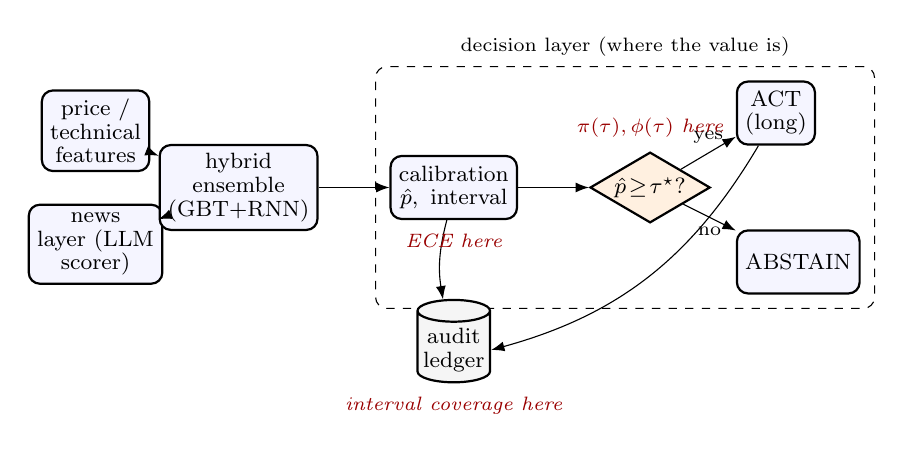
\begin{tikzpicture}[
  font=\footnotesize,
  box/.style={rectangle,rounded corners,draw,thick,align=center,inner sep=3pt,minimum height=8mm,fill=blue!4},
  gate/.style={diamond,draw,thick,align=center,inner sep=1pt,aspect=1.7,fill=orange!12},
  store/.style={cylinder,shape border rotate=90,aspect=0.3,draw,thick,align=center,inner sep=2pt,fill=gray!8},
  meas/.style={font=\scriptsize\itshape,red!60!black},
  >=Latex
]
\node[box] (px) {price /\\technical\\features};
\node[box,below=4mm of px] (news) {news\\layer (LLM\\scorer)};
\node[box,right=8mm of $(px)!0.5!(news)$] (ens) {hybrid\\ensemble\\(GBT+RNN)};
\node[box,right=9mm of ens] (cal) {calibration\\$\Pup,\ \text{interval}$};
\node[gate,right=9mm of cal] (g) {$\Pup\!\ge\!\tau^\star$?};
\node[box,above right=3mm and 7mm of g] (act) {ACT\\(long)};
\node[box,below right=3mm and 7mm of g] (ab) {ABSTAIN};
\node[store,below=10mm of cal] (led) {audit\\ledger};
\draw[->] (px)--(ens); \draw[->] (news)--(ens);
\draw[->] (ens)--(cal); \draw[->] (cal)--(g);
\draw[->] (g)-- node[above,font=\scriptsize]{yes} (act);
\draw[->] (g)-- node[below,font=\scriptsize]{no} (ab);
\draw[->] (cal) to[bend right=12] (led);
\draw[->] (act) to[bend left=22] (led.east);
\node[meas,below=0.5mm of cal] {ECE here};
\node[meas,above=0.5mm of g] {$\pi(\tau),\phi(\tau)$ here};
\node[meas,below=0.5mm of led] {interval coverage here};
\begin{scope}[on background layer]
\node[draw,dashed,rounded corners,fit=(cal)(g)(act)(ab),inner sep=5pt,label=above:{\scriptsize decision layer (where the value is)}] {};
\end{scope}
\end{tikzpicture}}
\caption{The deployed pipeline and where each measurement in
Section~\ref{sec:results} is taken. Features (price and news) feed a hybrid ensemble;
its directional probability is calibrated, then passed to a conviction gate that acts
or abstains; every issued forecast is written to an append-only ledger and later
scored against its target date. The dashed box is the decision layer the attribution
finds responsible for the realised value. The schematic is conceptual.}
\label{fig:pipeline}
\end{figure}

% =============================================================================
\section{Results: an account of where the value comes from}
\label{sec:results}
% =============================================================================
We now run the attribution procedure of Section~\ref{sec:procedure} on the deployed
system, in order.

\subsection{Deployed uncertainty does not self-correct}
\label{sec:resultcov}
We start with the live ledger because it sets the stakes. Between 19 April and 12
June 2026 the system issued and later resolved 621 price-interval forecasts on seven
NSE large caps (ABB, HDFCBANK, ICICIBANK, INFY, RELIANCE, SBIN, TCS), each carrying a
nominal 90\% interval with a median half-width of 5.6\% of price. Were the intervals
well calibrated, about 90\% should contain the realised price. They did not: empirical
coverage was 70.7\% overall, a 19.3 percentage-point shortfall. Most forecasts were at
the ten-day horizon, where coverage was 69.2\% over 575 resolved forecasts; the smaller
twenty-day and five-day buckets covered 86.8\% and 100\% (Table~\ref{tab:cov},
Figure~\ref{fig:cov}). Put plainly, realised prices broke through the $\pm5.6\%$ band
far more often than one time in ten, so the deployed model's stated confidence was
systematically overstated, and nothing in the pipeline noticed on its own. This is the
empirical reason calibration and abstention cannot be afterthoughts, and it is step one
of the attribution: before any value can be claimed, the uncertainty has to be shown to
be untrustworthy as shipped.

\begin{table}[t]
\caption{Live-ledger interval coverage by horizon (NSE large caps, 19 April--12 June
2026). All intervals carry a nominal 90\% level.}
\label{tab:cov}
\centering
\begin{tabular}{lccc}
\toprule
Horizon & Resolved forecasts & Nominal coverage & Empirical coverage \\
\midrule
5 trading days  & 8   & 90.0\% & 100.0\% \\
10 trading days & 575 & 90.0\% & 69.2\% \\
20 trading days & 38  & 90.0\% & 86.8\% \\
\midrule
All             & 621 & 90.0\% & 70.7\% \\
\bottomrule
\end{tabular}
\end{table}

\begin{figure}[t]
\centering
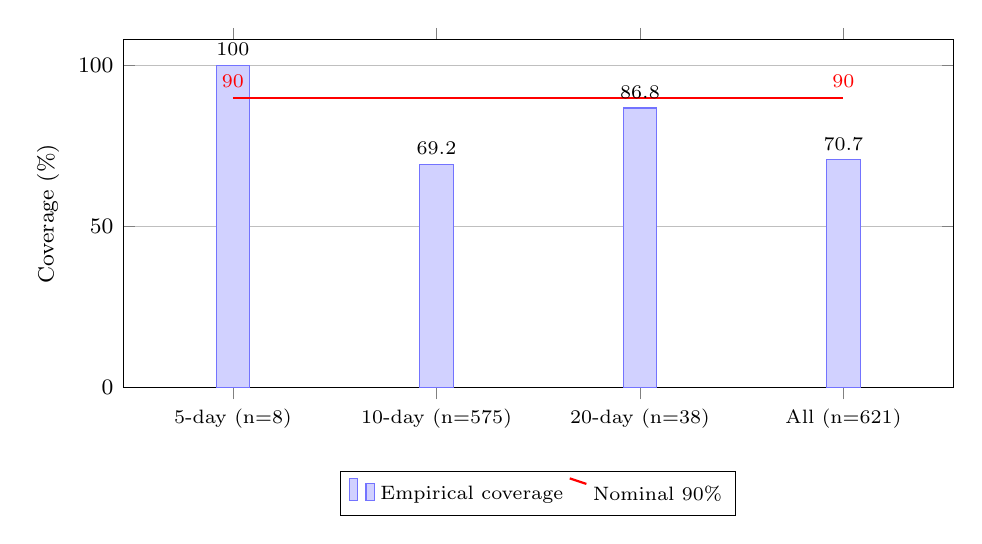
\begin{tikzpicture}
\begin{axis}[
  width=\linewidth, height=6.0cm, font=\footnotesize,
  ybar, bar width=12pt,
  symbolic x coords={5-day (n=8),10-day (n=575),20-day (n=38),All (n=621)},
  xtick=data, x tick label style={font=\scriptsize},
  ymin=0, ymax=108, ylabel={Coverage (\%)},
  enlarge x limits=0.18, ymajorgrids,
  legend style={at={(0.5,-0.24)},anchor=north,legend columns=2,font=\scriptsize},
  nodes near coords, every node near coord/.append style={font=\scriptsize}
]
\addplot[fill=blue!18,draw=blue!55] coordinates {(5-day (n=8),100.0)(10-day (n=575),69.2)(20-day (n=38),86.8)(All (n=621),70.7)};
\addplot[sharp plot,thick,red,mark=none,update limits=false] coordinates {(5-day (n=8),90)(All (n=621),90)};
\legend{Empirical coverage, Nominal 90\%}
\end{axis}
\end{tikzpicture}
\caption{Empirical coverage of nominal 90\% price intervals on the live ledger, by
horizon. The deployed intervals are materially under-covered at the dominant ten-day
horizon, which carries 575 of the 621 forecasts.}
\label{fig:cov}
\end{figure}

\subsection{The calibration term: a stacking bug, and a three-stage repair}
\label{sec:resultcal}
The offline diagnosis of overconfidence is sharper still; this and the two results
that follow are walk-forward measurements, not live-ledger figures. The deployed
model's next-day directional head reported probabilities clustered near 0.80 against a
realised accuracy of about 0.51, giving $\ece=0.345$ and a Brier score above 0.366,
worse than always predicting 0.5. Tracing the pipeline exposed a textbook
stacked-generalisation trap [Wolpert 1992]: an isotonic calibrator had been fitted on
the out-of-fold \emph{average of the base learners} but then applied to the
\emph{stacked} prediction, a different distribution, and the final blend carried no
calibration of its own. The fix is mechanical. We refit the isotonic map on the same
base-average it was meant to correct, form the blend, then fit a final Platt scaler
[Platt 1999] on a held-out fold and apply it to both the test rows and the live row.
This cut $\ece$ from 0.345 to 0.049 and pulled the reported up-probability back to a
realistic neighbourhood of 0.50.

The crucial observation, and the reason this is step two of the attribution rather than
a contribution in its own right, is that \emph{accuracy did not move}. The
recalibration map is monotone, so by the argument of Section~\ref{sec:decomp} it cannot
change the model's ordering of names, its accuracy, its AUC or its conviction lift. It
changed only the calibration gap, pulling the advertised probability onto the delivered
one. In decision-value terms, calibration did not create value; it made the value that
selection would later extract \emph{collectible}, by ensuring that the threshold
$\tau^\star$ would mean what it was set to mean. A system shipped at $\ece=0.345$ would
have a conviction gate firing on a probability scale that lies by 30 points; the gate
would be tuned on a fiction. The episode is also a clean, transferable lesson: a
calibrator is bound to the distribution it was fitted on, and stacking quietly creates
more than one such distribution.

\subsection{The ranking term is essentially zero}
\label{sec:ceiling}
Once calibration was repaired, it exposed an uncomfortable fact that the inflated
probabilities had hidden. With $\Pup$ pulled back to the base rate, we asked directly whether any robust
single-name directional edge survives at short horizons. A cross-sectional model
predicting five-day direction across the universe reached 50.09\% out-of-fold accuracy
on 131{,}809 ticker-days, with ranking AUC near 0.49, which is chance. We confirmed the result
five ways, varying the learner and the feature set and gating by trend and by market
regime: a per-ticker ensemble, a cross-sectional logistic model, a gradient-boosted
model with reversion features, trend/momentum gating, and market-regime gating. None
produced a stable edge over the always-up base rate at the daily scale; in this
sample the trend-gated variants sat \emph{below} the base rate, the universe being
mildly mean-reverting at that horizon. This is consistent with the efficient-market
prediction for liquid names [Fama 1970, Malkiel 2003], and it is step three of the
attribution: the ranking term that accuracy and AUC are built to reward is, here,
absent. By Proposition~\ref{prop:tail}, that absence does not by itself condemn the
system (an edge can still live in the tail), but it does mean that any value we find
must be a tail property, and cannot be a ranking one.

\subsection{The selection term carries a small, stable edge}
\label{sec:swing}
Lengthening the horizon to thirty trading days (about a month and a half, the use case
the product is actually sold for) opens two modest edges: the upward drift of
equities, since about 58\% of thirty-day windows are up, and a small idiosyncratic
component that a calibrated cross-sectional model can find on momentum, trend,
reversal and volatility features. Walk-forward from 2018 to 2026 over the 54-name
universe (91{,}471 training rows, 50{,}272 out-of-sample rows), the conviction gate of
\eqref{eq:tau} settles at $\tau^\star=0.63$. Its fired UP bucket achieves 60.6\%
directional precision against a 58.0\% always-up base,\footnote{The pooled base of
$58.0\%$ is the unconditional out-of-sample up-rate over all $50{,}272$ rows (the
always-act comparator $b$ of Definition~\ref{def:dv}), not the fires-weighted mean of
the per-year bases in Table~\ref{tab:year}, which is $55.9\%$. The unconditional rate
is the more conservative comparator; measured against the fires-weighted base the
pooled edge would read $+4.7$ points instead of $+2.6$.} a selection value of
$\sigma(\tau^\star)=+2.6$ percentage points, while firing on only 5.65\% of
observations; the gate abstains on the remaining 94\%. The fired bucket pools to
2{,}840 calls, so the 60.6\% precision carries a 95\% binomial interval of
58.8--62.4\%; a one-sided test against the 58.0\% base gives $z\approx2.8$
($p\approx0.003$), so the pooled edge is distinguishable from the base at conventional
levels. Whether this clears cost is the net-of-cost question of \eqref{eq:dv}. We lack
position-level fills to compute $V$ exactly, but the order of magnitude is reassuring:
at a thirty-day horizon the typical absolute move in these names runs to several per
cent, against a round-trip cost of order $0.2\%$ for liquid large caps, so a
long/abstain edge of $2.6$ points is not erased by friction. A precise $V$ awaits
position-level accounting, which we flag among the limitations.

We do not over-read it. The per-year fired counts are small (Table~\ref{tab:year}), so
the year-to-year swings, from $+10.8$ points in 2025 to $-2.4$ in 2024, are within
sampling noise, and the fair summary is a small but repeatable tail edge rather than
a strong one. The gate beats its base rate in four of the five test years
(Figure~\ref{fig:year}); the single exception, 2024, sits in the table with the rest.
The ranking AUC of this signal is about 0.47, at or below chance, which is the
regime Proposition~\ref{prop:tail} describes: the edge lives in the high-conviction
tail and not in the ordering, so precision at a fixed firing rate registers it while
AUC overlooks it. Confident DOWN calls, for completeness, reach only about 10\%
precision out-of-sample, destroyed by drift, which is why the gate is one-sided and
never emits them.

\begin{table}[t]
\caption{Walk-forward selective signal, by test year. Precision is the realised
up-rate of the fired high-conviction bucket; base is the always-up rate that year;
fires is the number of high-conviction calls that year.}
\label{tab:year}
\centering
\begin{tabular}{lcccc}
\toprule
Test year & Fires & Fired-bucket precision & Always-up base & Edge (pp) \\
\midrule
2022 & 365 & 61.6\% & 54.0\% & $+7.6$ \\
2023 & 290 & 68.3\% & 65.3\% & $+3.0$ \\
2024 & 932 & 53.3\% & 55.7\% & $-2.4$ \\
2025 & 822 & 69.0\% & 58.2\% & $+10.8$ \\
2026 & 431 & 54.5\% & 47.1\% & $+7.4$ \\
\midrule
Pooled & 2{,}840 & 60.6\% & 58.0\% & $+2.6$ \\
\bottomrule
\end{tabular}
\end{table}

\begin{figure}[t]
\centering
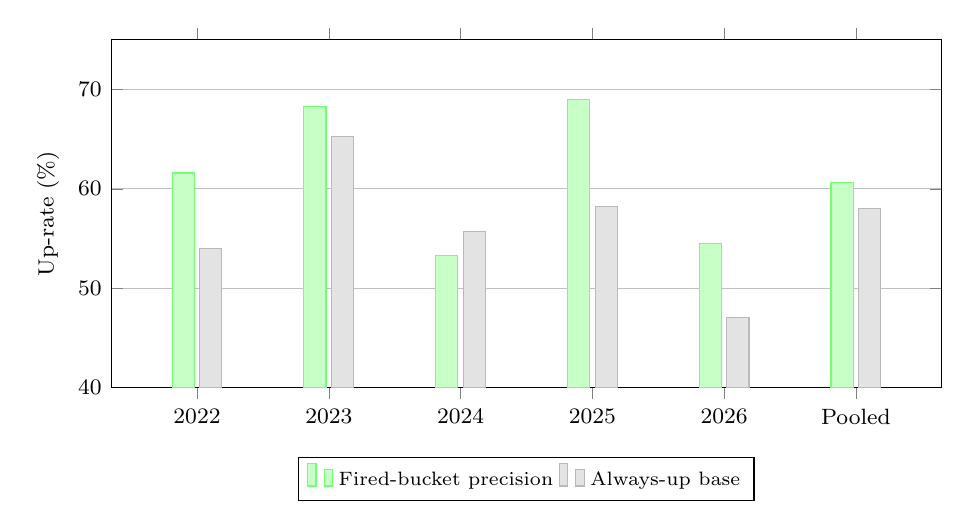
\begin{tikzpicture}
\begin{axis}[
  width=\linewidth, height=6.0cm, font=\footnotesize,
  ybar, bar width=8pt,
  symbolic x coords={2022,2023,2024,2025,2026,Pooled},
  xtick=data, ymin=40, ymax=75, ylabel={Up-rate (\%)},
  enlarge x limits=0.13, ymajorgrids,
  legend style={at={(0.5,-0.2)},anchor=north,legend columns=2,font=\scriptsize}
]
\addplot[fill=green!22,draw=green!55] coordinates {(2022,61.6)(2023,68.3)(2024,53.3)(2025,69.0)(2026,54.5)(Pooled,60.6)};
\addplot[fill=gray!22,draw=gray!55] coordinates {(2022,54.0)(2023,65.3)(2024,55.7)(2025,58.2)(2026,47.1)(Pooled,58.0)};
\legend{Fired-bucket precision, Always-up base}
\end{axis}
\end{tikzpicture}
\caption{Selective signal versus its base rate by test year. The conviction gate beats
the always-up base in four of five years and pooled, while firing on about 5.6\% of
observations.}
\label{fig:year}
\end{figure}

\subsection{Settling the attribution}
\label{sec:attrib}
We can now state, in measured numbers, where the realised decision value comes from.
The system's only positive, collectible edge is the fired precision of its conviction
gate, $\pi(\tau^\star)=60.6\%$. By the decomposition \eqref{eq:partition} and
Definition~\ref{def:dv} this splits cleanly into the components the four preceding
subsections measured, summarised in Table~\ref{tab:attrib} and drawn as a waterfall in
Figure~\ref{fig:waterfall}.

\begin{table}[t]
\caption{Decision-value attribution of the deployed system. Each row is a measured
quantity from Sections~\ref{sec:resultcov}--\ref{sec:swing}; the realised fired
precision is the sum of the drift base and the selection value, with ranking and
calibration acting as described.}
\label{tab:attrib}
\centering
\begin{tabular}{p{4.9cm}p{2.6cm}p{4.6cm}}
\toprule
Component & Measured value & Role in decision value \\
\midrule
Drift (base rate $b$) & 58.0\% up-rate & Beta, not skill; available with no model. \\[2pt]
Selection value $\sigma(\tau^\star)$ & $+2.6$ pp & The only positive, collectible edge; a tail property. \\[2pt]
Ranking skill (AUC$-\tfrac12$) & $-0.01$ to $-0.03$ & Daily $\approx\!-0.01$, 30-day $\approx\!-0.03$; invisible to selection (Prop.~\ref{prop:tail}). \\[2pt]
Calibration ($\ece$) & $0.345\!\to\!0.049$ & Enabling, not additive; makes $\tau^\star$ trustworthy. \\[2pt]
Deployed interval coverage & $70.7\%$ vs $90\%$ nominal & The risk the attribution exists to expose. \\
\midrule
Realised fired precision $\pi(\tau^\star)$ & $60.6\%=b+\sigma$ & What the system can actually be paid for. \\
\bottomrule
\end{tabular}
\end{table}

\begin{figure}[t]
\centering
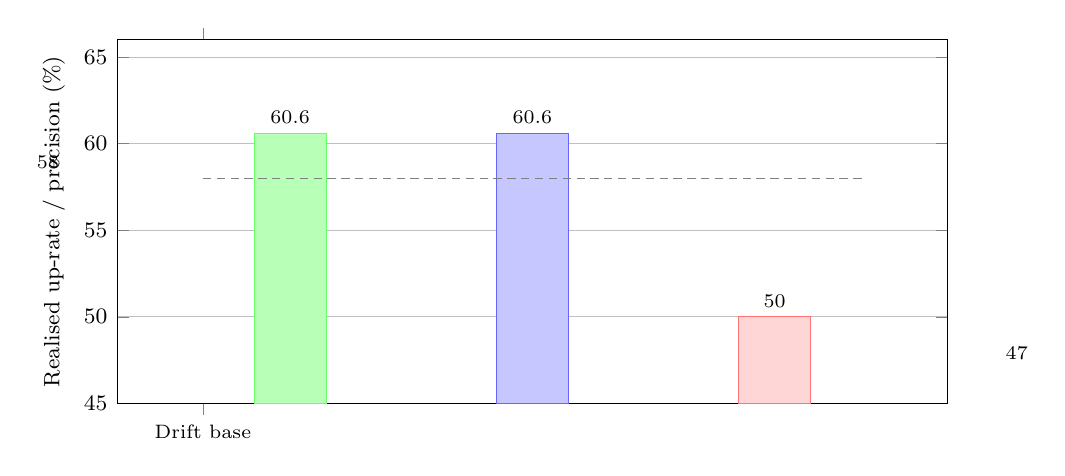
\begin{tikzpicture}
\begin{axis}[
  width=\linewidth, height=6.2cm, font=\footnotesize,
  ybar, bar width=26pt,
  symbolic x coords={Drift base,Selection,Fired prec.,Ranking acc.,AUC read.},
  xtick=data, x tick label style={font=\scriptsize},
  ymin=45, ymax=66, ylabel={Realised up-rate / precision (\%)},
  enlarge x limits=0.13, ymajorgrids,
  nodes near coords, every node near coord/.append style={font=\scriptsize},
]
\addplot[fill=gray!25,draw=gray!60] coordinates {(Drift base,58.0)};
\addplot[fill=green!28,draw=green!60] coordinates {(Selection,60.6)};
\addplot[fill=blue!22,draw=blue!60] coordinates {(Fired prec.,60.6)};
\addplot[fill=red!16,draw=red!55] coordinates {(Ranking acc.,50.0)};
\addplot[fill=red!10,draw=red!45] coordinates {(AUC read.,47.0)};
\draw[densely dashed,gray] (axis cs:Drift base,58.0) -- (axis cs:AUC read.,58.0);
\end{axis}
\end{tikzpicture}
\caption{Decision-value waterfall. The drift base (58.0\%) plus the selection value of
the conviction gate ($+2.6$ pp) account for the realised fired precision (60.6\%). The
two right-hand bars show what the conventional scorecard reports for the same signal,
and are not up-rates: directional accuracy at chance (50.0\%) and a ranking AUC of
about 0.47 (plotted as AUC$\times100$ for comparison), neither of which sees the
tail edge. The dashed line marks the drift base. All values are measured
(Sections~\ref{sec:ceiling}--\ref{sec:swing}).}
\label{fig:waterfall}
\end{figure}

The split is clean. Of the 60.6 points of realised fired precision, 58.0 are
drift (a market beta any index fund collects), and 2.6 are the selection value the
system adds. The ranking term that accuracy (50.0\%) and AUC ($\approx0.47$) measure
contributes nothing; on the standard scorecard this signal is a failure, and a
practitioner who graded it that way would discard a small but statistically
distinguishable edge. Calibration appears nowhere as an additive term, just as
Section~\ref{sec:decomp} predicts, and yet without the repair from $\ece=0.345$ to
$0.049$ the conviction threshold would have been set on a lying probability scale and
the 2.6-point edge would not have been collectible. So the account says three things at
once. The model's prediction is not where the value sits. Selection is. And calibration
is the precondition that lets the selection edge be banked. Table~\ref{tab:attrib}
captures the economics of this system, and the pattern, we argue next, is not peculiar
to it.

% =============================================================================
\section{Discussion}
\label{sec:discussion}
% =============================================================================
\subsection{What the attribution generalises to}
The numbers are from one platform; the shape of the attribution is not. Any deployed
forecaster that decides whether to act, in a domain where the base rate is high and
the ordering signal is weak, will show a similar profile: a large beta-like base, a
thin selection edge in the tail, a calibration term that enables rather than adds, and
a ranking term the standard scorecard over-weights. Markets are the cleanest example
because their efficiency drives the ranking term toward zero [Fama 1970,
Malkiel 2003] and their outcomes are public and unforgiving, but the structure recurs
wherever a model triages a stream of opportunities and is judged on the few it picks.
The recommendation that follows is concrete and portable, and we set it out as a
reporting checklist in Section~\ref{sec:checklist}. A great deal of financial-ML work
optimises the ranking term, which our results suggest is the one term least likely to
survive deployment.

\subsection{Why the standard scorecard misleads, restated}
Proposition~\ref{prop:tail} carries the generalisation. Accuracy and AUC summarise
global behaviour. A selective system is defined by what happens in a thin tail. The two
are provably decoupled. This is not a quirk of our data. It is why a
literature that reports AUC can simultaneously be full of models that look skilful and
empty of models that deploy: the metric rewards a property (global ordering) that is
both easy to overfit in backtests [Bailey et al.\ 2017, Harvey et al.\ 2016] and
largely irrelevant to a system that acts on its tail. Reporting precision at coverage,
as the selective-prediction community does [Geifman and El-Yaniv 2017,
El-Yaniv and Wiener 2010], aligns the metric with the deployment. The decision-value
account grades a model on the trades it would actually make.

\subsection{Threats to validity and limits}
Five limits deserve emphasis. First, the live ledger is young, just two months and seven
names, so its 19.3-point coverage shortfall, though large and consistent at the
dominant horizon, is a current snapshot rather than a stationary law, and the
directional-probability sample on the ledger is still too small (28 resolved
next-period calls) to support a live reliability diagram; our live claim therefore
rests on the 621-forecast interval-coverage evidence, and the calibration and selection
results are offline walk-forward measurements. Second, the selection edge is small in
absolute terms (2.6 points) and its per-year variation is within sampling noise; we
report it as a thin, repeatable tail edge and explicitly not as a strong signal.
Third, the news layer's contribution is argued from its place in the pipeline and not
from an isolated backtest, because the deployment does not store per-event return
labels; we prefer to say this plainly than to reconstruct a clean number, which is the
kind of exercise the backtest-overfitting critique exists to catch. Fourth, the
calibration drifts over time and must be maintained on a schedule; we treat the
maintenance question as out of scope here and a matter for separate work, and make no
claim about an optimal recalibration cadence in this paper. Fifth, we attribute the
cost-free selection value $\sigma$ rather than the full net-of-cost decision value $V$
of \eqref{eq:dv}; the order-of-magnitude argument of Section~\ref{sec:swing} suggests
the edge survives friction, but a position-level computation of $V$ from realised fills
and sizing is left for future work.

\subsection{Reporting decision value: a short checklist}
\label{sec:checklist}
The attribution is easy to adopt, so we state it as a checklist a practitioner can run
against any deployed selective forecaster. Publish a coverage audit first: take the live
ledger, compare nominal with empirical interval coverage, and report the gap by horizon,
as in Table~\ref{tab:cov}. Report calibration before and after any post-hoc fix, with
the expected calibration error and a note that accuracy did not move, which certifies
the fix touched only reliability. State the base rate $b$ explicitly and compare the
fired bucket against it, not against an even-odds prior; the drift in a long-only equity
setting is large, and it is not skill. Report precision at a fixed firing rate,
$\pi(\tau)$ at $\phi(\tau)$, with a confidence interval and a test against $b$, in place
of accuracy or AUC. Separate the ranking term: give the AUC, and if it sits near or
below one half while tail precision is positive, say so, because that pattern is the
signature of a tail-only edge. Finally, where costs are known, convert the selection
value to a net-of-cost figure through \eqref{eq:dv}; where they are not, scope the claim
to the cost-free core and name the quantity being reported. A paper that fills in these
six lines is hard to misread, and a system that cannot fill them in is not yet ready to
be trusted with a position.

\subsection{Relation to selective and conformal prediction}
The conviction gate is an instance of selective classification [Chow 1970,
Geifman and El-Yaniv 2017]; what the decision-value account adds is the attribution,
separating the gate's selection value from the drift it rides on and the calibration
that makes it bankable, together with the tail--AUC result that justifies measuring it at a
fixed firing rate. The interval under-coverage we documented in
Section~\ref{sec:resultcov} is the failure that distribution-free methods are
built to address; adaptive conformal inference [Gibbs and Cand\`es 2021,
Angelopoulos and Bates 2021] is designed for this kind of non-stationary
coverage shortfall, and replacing the deployed parametric intervals with an adaptive
conformal layer is the clearest next step the attribution points to.

% =============================================================================
\section{Conclusion}
\label{sec:conclusion}
% =============================================================================
Machine-learning systems for markets are usually graded on accuracy and AUC, and most
of them, graded carefully, have neither. We have argued that this is the wrong way to
keep score. A deployed forecaster is paid for the quality of the positions it actually
takes, weighed against those it skips, and we made that quantity, its decision value,
precise by extending the calibration--refinement and reliability--resolution
decompositions of forecast verification into the abstaining, cost-aware decision
setting. The framework comes with a theorem that explains why the usual scorecard
cannot see what such a system is worth: selection value lives in the tail of the score
distribution and is provably decoupled from global AUC, so a system with real decision
value can be reported at chance. We then ran the attribution on a live equity platform.
The result is uncomfortable, and we believe it is representative. Deployed 90\%
intervals covered only 70.7\% of outcomes, so confidence had to be earned rather than
assumed; a calibration repair cut expected calibration error from 0.35 to 0.05 without
adding a point of accuracy; single-name direction proved unpredictable beyond drift;
and a conviction gate that abstains on 94\% of names nonetheless banked a 60.6\% hit
rate against a 58.0\% base, in four of five years. Drift is just beta. The edge comes
from selection. Calibration is the precondition that makes it bankable. And
prediction, the thing the field optimises for, contributes almost nothing. The
practical message follows: instrument the uncertainty layer, grade the model on the
trades it would make, and put the engineering effort where the attribution says the
value is. Replacing the deployed intervals with an adaptive conformal layer, and a
per-event labelled evaluation of the news contribution, are the clear next steps.

% ----------------------------------------------------------------------------
\section*{Acknowledgements}
The authors thank the Department of Computer Engineering, Fr.\ C.\ Rodrigues Institute
of Technology, for computing support. The list of authors and their contributions is
consistent with the CRediT taxonomy entered with the submission.

\section*{Declaration of generative AI and AI-assisted technologies}
Two distinct uses are disclosed. (i) \emph{As an instrument within the system under
study}: an instruction-tuned large language model (Claude Haiku 4.5, Anthropic) scores
news headlines for the feature layer described in Section~\ref{sec:news}, from the
anchored prompt summarised there; these outputs are part of the deployed pipeline,
were validated against a deterministic lexicon fallback, and are persisted for audit.
(ii) \emph{In manuscript preparation}: during the writing of this paper the authors
used a large language model solely to improve the language and readability of
author-written drafts. No generative tool produced data, results, figures or
interpretations; every quantitative finding derives from the authors' deployed system
and its measured ledger. After using these tools the authors reviewed and edited the
content and take full responsibility for the publication.

\section*{Data availability}
The live forecast ledger and the offline walk-forward statistics underlying
Tables~\ref{tab:cov}--\ref{tab:attrib} and Figures~\ref{fig:cov}--\ref{fig:waterfall}
can be made available by the corresponding author on reasonable request, subject to the
platform's terms. Source price data are public NSE end-of-day records.

\section*{Conflict of interest}
The authors declare that they have no conflict of interest.

% ----------------------------------------------------------------------------
% References in J.UCS [Author Year] style. Every entry is a real, citeable work.
% ----------------------------------------------------------------------------
{\fontsize{9}{11}\selectfont
\begin{thebibliography}{Niculescu-Mizil and Caruana 2005}
\setlength{\itemsep}{1pt}

\bibitem[Angelopoulos and Bates 2021]{angelopoulos2021}
Angelopoulos, A.\ N., Bates, S.: ``A gentle introduction to conformal prediction and
distribution-free uncertainty quantification''; arXiv:2107.07511 (2021).
doi:10.48550/arXiv.2107.07511

\bibitem[Antweiler and Frank 2004]{antweiler2004}
Antweiler, W., Frank, M.\ Z.: ``Is all that talk just noise? The information content of
internet stock message boards''; The Journal of Finance, 59, 3 (2004), 1259--1294.
doi:10.1111/j.1540-6261.2004.00662.x

\bibitem[Bailey et al.\ 2017]{bailey2017}
Bailey, D.\ H., Borwein, J., Lopez de Prado, M., Zhu, Q.\ J.: ``The probability of
backtest overfitting''; Journal of Computational Finance, 20, 4 (2017), 39--69.
doi:10.21314/JCF.2016.322

\bibitem[Brier 1950]{brier1950}
Brier, G.\ W.: ``Verification of forecasts expressed in terms of probability''; Monthly
Weather Review, 78, 1 (1950), 1--3.
doi:10.1175/1520-0493(1950)078<0001:VOFEIT>2.0.CO;2

\bibitem[Chow 1970]{chow1970}
Chow, C.\ K.: ``On optimum recognition error and reject tradeoff''; IEEE Transactions
on Information Theory, 16, 1 (1970), 41--46. doi:10.1109/TIT.1970.1054406

\bibitem[DeGroot and Fienberg 1983]{degroot1983}
DeGroot, M.\ H., Fienberg, S.\ E.: ``The comparison and evaluation of forecasters'';
Journal of the Royal Statistical Society: Series D (The Statistician), 32, 1--2 (1983),
12--22. doi:10.2307/2987588

\bibitem[Devlin et al.\ 2019]{devlin2019}
Devlin, J., Chang, M.\ W., Lee, K., Toutanova, K.: ``BERT: pre-training of deep
bidirectional transformers for language understanding''; Proc.\ NAACL-HLT 2019,
Minneapolis, MN, USA (2019), 4171--4186. doi:10.18653/v1/N19-1423

\bibitem[El-Yaniv and Wiener 2010]{elyaniv2010}
El-Yaniv, R., Wiener, Y.: ``On the foundations of noise-free selective
classification''; Journal of Machine Learning Research, 11 (2010), 1605--1641.

\bibitem[Fama 1970]{fama1970}
Fama, E.\ F.: ``Efficient capital markets: a review of theory and empirical work'';
The Journal of Finance, 25, 2 (1970), 383--417. doi:10.2307/2325486

\bibitem[Fischer and Krauss 2018]{fischer2018}
Fischer, T., Krauss, C.: ``Deep learning with long short-term memory networks for
financial market predictions''; European Journal of Operational Research, 270, 2
(2018), 654--669. doi:10.1016/j.ejor.2017.11.054

\bibitem[Geifman and El-Yaniv 2017]{geifman2017}
Geifman, Y., El-Yaniv, R.: ``Selective classification for deep neural networks'';
Advances in Neural Information Processing Systems 30 (NeurIPS 2017), Long Beach, CA,
USA (2017), 4878--4887.

\bibitem[Gibbs and Cand\`es 2021]{gibbs2021}
Gibbs, I., Cand\`es, E.: ``Adaptive conformal inference under distribution shift'';
Advances in Neural Information Processing Systems 34 (NeurIPS 2021) (2021),
1660--1672.

\bibitem[Gneiting and Raftery 2007]{gneitingraftery2007}
Gneiting, T., Raftery, A.\ E.: ``Strictly proper scoring rules, prediction, and
estimation''; Journal of the American Statistical Association, 102, 477 (2007),
359--378. doi:10.1198/016214506000001437

\bibitem[Gneiting et al.\ 2007]{gneiting2007}
Gneiting, T., Balabdaoui, F., Raftery, A.\ E.: ``Probabilistic forecasts, calibration
and sharpness''; Journal of the Royal Statistical Society: Series B, 69, 2 (2007),
243--268. doi:10.1111/j.1467-9868.2007.00587.x

\bibitem[Granger and Pesaran 2000]{granger2000}
Granger, C.\ W.\ J., Pesaran, M.\ H.: ``Economic and statistical measures of forecast
accuracy''; Journal of Forecasting, 19, 7 (2000), 537--560.
doi:10.1002/1099-131X(200012)19:7<537::AID-FOR769>3.0.CO;2-G

\bibitem[Gu et al.\ 2020]{gu2020}
Gu, S., Kelly, B., Xiu, D.: ``Empirical asset pricing via machine learning''; The
Review of Financial Studies, 33, 5 (2020), 2223--2273. doi:10.1093/rfs/hhaa009

\bibitem[Guo et al.\ 2017]{guo2017}
Guo, C., Pleiss, G., Sun, Y., Weinberger, K.\ Q.: ``On calibration of modern neural
networks''; Proc.\ 34th International Conference on Machine Learning (ICML 2017),
Sydney, Australia (2017), 1321--1330.

\bibitem[Harvey et al.\ 2016]{harvey2016}
Harvey, C.\ R., Liu, Y., Zhu, H.: ``$\ldots$ and the cross-section of expected
returns''; The Review of Financial Studies, 29, 1 (2016), 5--68.
doi:10.1093/rfs/hhv059

\bibitem[Jiang 2021]{jiang2021}
Jiang, W.: ``Applications of deep learning in stock market prediction: recent
progress''; Expert Systems with Applications, 184 (2021), 115537.
doi:10.1016/j.eswa.2021.115537

\bibitem[Ke et al.\ 2019]{ke2019}
Ke, Z.\ T., Kelly, B.\ T., Xiu, D.: ``Predicting returns with text data''; National
Bureau of Economic Research Working Paper 26186, Cambridge, MA, USA (2019).
doi:10.3386/w26186

\bibitem[Krauss et al.\ 2017]{krauss2017}
Krauss, C., Do, X.\ A., Huck, N.: ``Deep neural networks, gradient-boosted trees,
random forests: statistical arbitrage on the S\&P 500''; European Journal of
Operational Research, 259, 2 (2017), 689--702. doi:10.1016/j.ejor.2016.10.031

\bibitem[Lopez de Prado 2018]{lopezdeprado2018}
Lopez de Prado, M.: ``Advances in Financial Machine Learning''; Wiley, Hoboken, NJ,
USA (2018).

\bibitem[Lopez-Lira and Tang 2023]{lopezlira2023}
Lopez-Lira, A., Tang, Y.: ``Can ChatGPT forecast stock price movements? Return
predictability and large language models''; arXiv:2304.07619 (2023).
doi:10.48550/arXiv.2304.07619

\bibitem[Loughran and McDonald 2011]{loughran2011}
Loughran, T., McDonald, B.: ``When is a liability not a liability? Textual analysis,
dictionaries, and 10-Ks''; The Journal of Finance, 66, 1 (2011), 35--65.
doi:10.1111/j.1540-6261.2010.01625.x

\bibitem[Malkiel 2003]{malkiel2003}
Malkiel, B.\ G.: ``The efficient market hypothesis and its critics''; Journal of
Economic Perspectives, 17, 1 (2003), 59--82. doi:10.1257/089533003321164958

\bibitem[Murphy 1973]{murphy1973}
Murphy, A.\ H.: ``A new vector partition of the probability score''; Journal of Applied
Meteorology, 12, 4 (1973), 595--600.
doi:10.1175/1520-0450(1973)012<0595:ANVPOT>2.0.CO;2

\bibitem[Murphy 1993]{murphy1993}
Murphy, A.\ H.: ``What is a good forecast? An essay on the nature of goodness in weather
forecasting''; Weather and Forecasting, 8, 2 (1993), 281--293.
doi:10.1175/1520-0434(1993)008<0281:WIAGFA>2.0.CO;2

\bibitem[Naeini et al.\ 2015]{naeini2015}
Naeini, M.\ P., Cooper, G.\ F., Hauskrecht, M.: ``Obtaining well calibrated
probabilities using Bayesian binning''; Proc.\ 29th AAAI Conference on Artificial
Intelligence, Austin, TX, USA (2015), 2901--2907.

\bibitem[Niculescu-Mizil and Caruana 2005]{niculescu2005}
Niculescu-Mizil, A., Caruana, R.: ``Predicting good probabilities with supervised
learning''; Proc.\ 22nd International Conference on Machine Learning (ICML 2005),
Bonn, Germany (2005), 625--632. doi:10.1145/1102351.1102430

\bibitem[Platt 1999]{platt1999}
Platt, J.\ C.: ``Probabilistic outputs for support vector machines and comparisons to
regularized likelihood methods''; in Smola, A.\ J., Bartlett, P., Sch\"olkopf, B.,
Schuurmans, D.\ (Eds.), Advances in Large Margin Classifiers, MIT Press, Cambridge,
MA, USA (1999), 61--74.

\bibitem[Sezer et al.\ 2020]{sezer2020}
Sezer, O.\ B., Gudelek, M.\ U., Ozbayoglu, A.\ M.: ``Financial time series forecasting
with deep learning: a systematic literature review: 2005--2019''; Applied Soft
Computing, 90 (2020), 106181. doi:10.1016/j.asoc.2020.106181

\bibitem[Sharpe 1994]{sharpe1994}
Sharpe, W.\ F.: ``The Sharpe ratio''; Journal of Portfolio Management, 21, 1 (1994),
49--58. doi:10.3905/jpm.1994.409501

\bibitem[Tetlock 2007]{tetlock2007}
Tetlock, P.\ C.: ``Giving content to investor sentiment: the role of media in the stock
market''; The Journal of Finance, 62, 3 (2007), 1139--1168.
doi:10.1111/j.1540-6261.2007.01232.x

\bibitem[Vovk et al.\ 2005]{vovk2005}
Vovk, V., Gammerman, A., Shafer, G.: ``Algorithmic Learning in a Random World'';
Springer, New York, NY, USA (2005).

\bibitem[Wolpert 1992]{wolpert1992}
Wolpert, D.\ H.: ``Stacked generalization''; Neural Networks, 5, 2 (1992), 241--259.
doi:10.1016/S0893-6080(05)80023-1

\bibitem[Zadrozny and Elkan 2002]{zadrozny2002}
Zadrozny, B., Elkan, C.: ``Transforming classifier scores into accurate multiclass
probability estimates''; Proc.\ 8th ACM SIGKDD International Conference on Knowledge
Discovery and Data Mining, Edmonton, Canada (2002), 694--699.
doi:10.1145/775047.775151

\end{thebibliography}
\par}

\end{document}
